 \chapter{\label{chap:intro}Análise Dos Resultados}
 




\section{Resultados da \textit{Survey}}

Após a conclusão do processo de coleta dados, com o objetivo de entender quais são as preocupações de desenvolvedores de software móveis no desenvolvimento de aplicações, destaca-se nessa seção o resultado obtido na survey. A survey teve um total de 20 respondentes.

O público que respondeu essa pesquisa tem em média 5 anos de experiência com desenvolvimento de aplicações  para dispositivos móveis e em sua maioria tem experiência com a plataforma Android. 

\begin{figure}
    \centering
    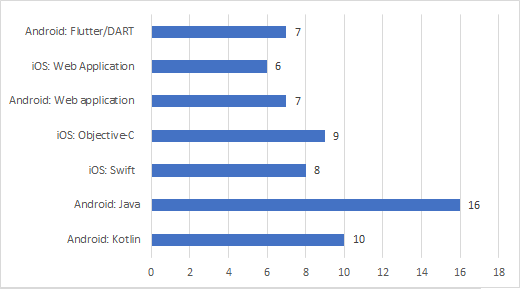
\includegraphics[scale=0.9]{fig/plataformas.PNG}
    \caption{Plataformas utilizadas pelos entrevistados}
    \label{fig:my_label}
\end{figure}



\begin{figure}[t]
\centering
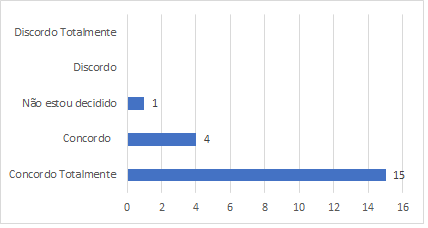
\includegraphics[scale=0.8]{figuras das questoes/1.1.PNG}
\caption{Preocupo-me com o controle de acesso de usuários nos sistemas que desenvolvo.}
\end{figure}


\begin{figure}[!t]
\centering
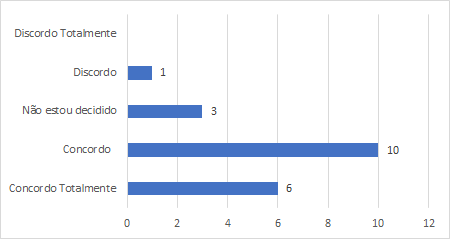
\includegraphics[scale=0.8]{figuras das questoes/1.2.PNG}
\caption{Preocupo-me em criar ou utilizar funcionalidades que permitam o bloqueio, remoção ou desabilitação rápida de usuários no sistema (por exemplo, funcionários que deixaram a empresa).}
\end{figure}

\begin{figure}[!t]
\centering
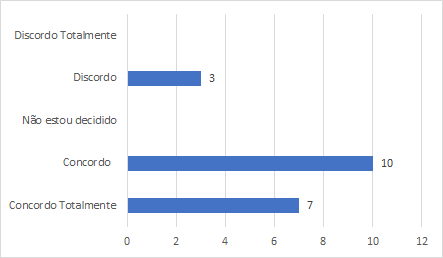
\includegraphics[scale=0.7]{figuras das questoes/1.3.png}
\caption{Preocupo-me em desenvolver funções que permitam a alteração de permissão no
sistema para todos os usuários, ou seja, que seja possível o gerenciamento de usuários.}
\end{figure}

\begin{figure}[!t]
\centering
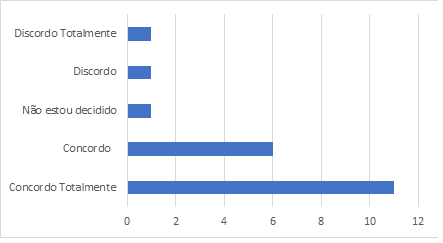
\includegraphics[scale=0.7]{figuras das questoes/1.4.png}
\caption{Preocupo-me em criar um registro central de direitos de acesso para cada usuário, ou seja, todos os usuários possuem um ID único.}
\end{figure}

\begin{figure}[!t]
\centering
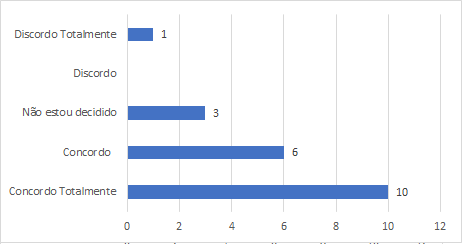
\includegraphics[scale=0.7]{figuras das questoes/2.1.png}
\caption{Preocupo-me em desenvolver funções que verifiquem a identidade de um usuário antes de fornecer uma informação de autenticação secreta, temporária, de substituição ou nova no sistema. (por exemplo e-mail de confirmação, SMS, aplicativos como Google autenticador).}
\end{figure}

\begin{figure}[!t]
\centering
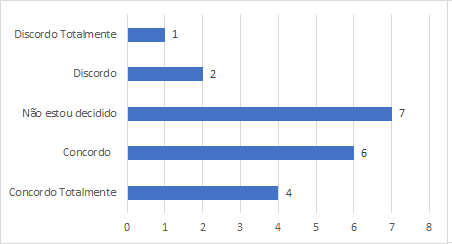
\includegraphics[scale=0.7]{figuras das questoes/2.2.png}
\caption{Preocupo-me em aprimorar o desenvolvimento de funcionalidades com autenticação secreta para acessos e logins. (autenticação por 2 fatores).}
\end{figure}

\begin{figure}[!t]
\centering
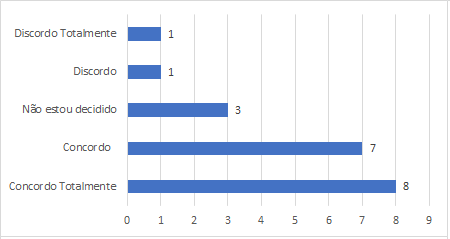
\includegraphics[scale=0.7]{figuras das questoes/2.3.png}
\caption{Preocupo-me para que a Informação de autenticação secreta temporária seja única para uma pessoa e que não possa ser facilmente adivinhada.}
\end{figure}

\begin{figure}[!t]
\centering
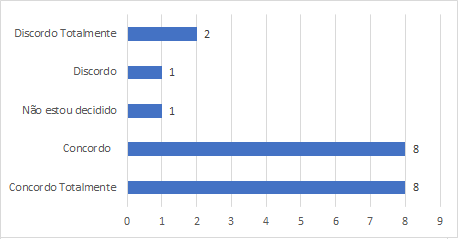
\includegraphics[scale=0.7]{figuras das questoes/2.4.png}
\caption{Preocupo-me em fornecer recursos para que o usuário consiga resguardar sua privacidade durante o processo de autenticação.}
\end{figure}

\begin{figure}[!t]
\centering
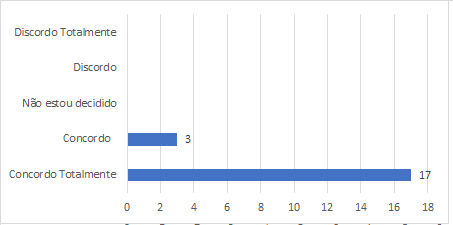
\includegraphics[scale=0.7]{figuras das questoes/2.5.png}
\caption{Preocupo-me em não mostrar dados sensíveis do usuário (status, informações pessoais, etc.) de aplicações até que o processo de Log-on tenha sido concluído com sucesso.}
\end{figure}

\begin{figure}[!t]
\centering
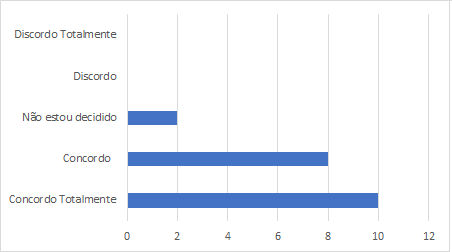
\includegraphics[scale=0.7]{figuras das questoes/2.6.png}
\caption{Preocupo-me em validar informações de entrada no sistema somente quando todos os dados de entrada estiverem completos.}
\end{figure}

\begin{figure}[!t]
\centering
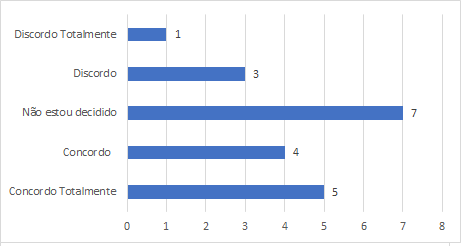
\includegraphics[scale=0.7]{figuras das questoes/2.7.png}
\caption{Caso ocorra um erro na validação das informações de entrada me preocupo em não identificar qual parte do dado de entrada está correto ou incorreto (Ex: “Sua senha está incorreta”).}
\end{figure}

\begin{figure}[!t]
\centering
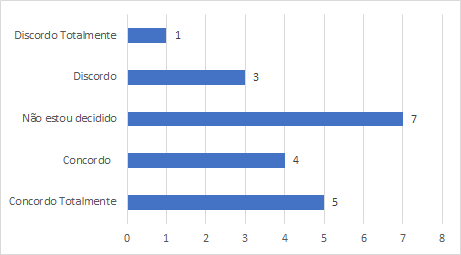
\includegraphics[scale=0.7]{figuras das questoes/2.8.png}
\caption{Preocupo-me em proteger o sistema contra tentativas consecutivas/repetidas de entrada forçada.}
\end{figure}

\begin{figure}[!t]
\centering
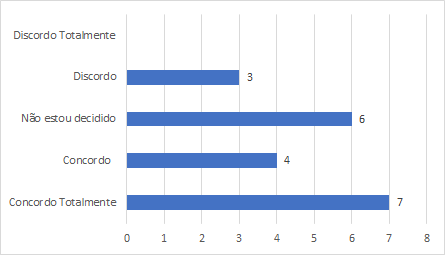
\includegraphics[scale=0.7]{figuras das questoes/2.9.png}
\caption{Preocupo-me em comunicar um evento de segurança caso uma tentativa potencial ou uma violação bem sucedida de entrada no sistema (log-on), seja detectada.}
\end{figure}

\begin{figure}[!t]
\centering
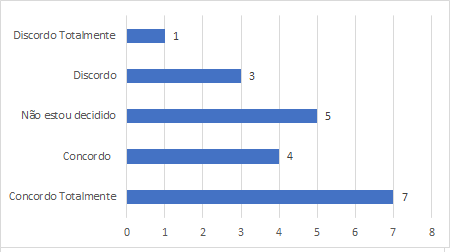
\includegraphics[scale=0.7]{figuras das questoes/2.10.png}
\caption{Preocupo-me em encerrar sessões inativas após um período de inatividade.}
\end{figure}

\begin{figure}[!t]
\centering
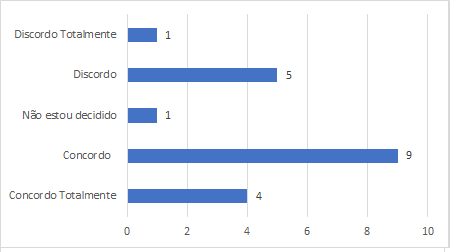
\includegraphics[scale=0.7]{figuras das questoes/2.11.png}
\caption{Preocupo-me em fazer sistemas que obriguem uma escolha de senha de qualidade, por exemplo, com no mínimo Oito Caracteres, misturar letras em caixa alta e baixa com números e caracteres não alfanuméricos).}
\end{figure}

\begin{figure}[!t]
\centering
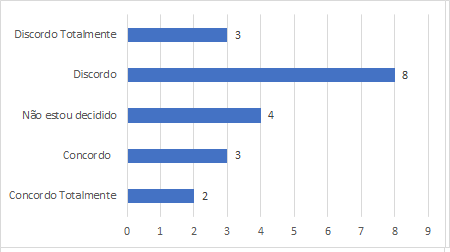
\includegraphics[scale=0.7]{figuras das questoes/2.12.png}
\caption{Preocupo-me em desenvolver sistemas que obriguem usuário a mudarem as suas senhas temporárias no primeiro acesso ao sistema (Sistema que coloca sua senha inicial como data de aniversário ou dígitos do RG).}
\end{figure}

\begin{figure}[!t]
\centering
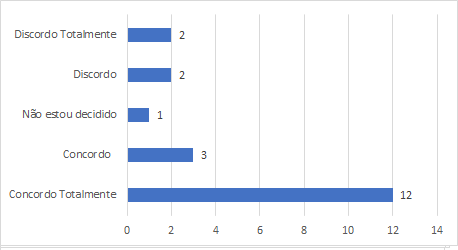
\includegraphics[scale=0.7]{figuras das questoes/2.13.png}
\caption{Preocupo-me em não permitir que a senhas possam ser mostradas na tela quando digitadas (Ex: Usar recurso do “olho” para revelar senha em um campo).}
\end{figure}

\begin{figure}[!t]
\centering
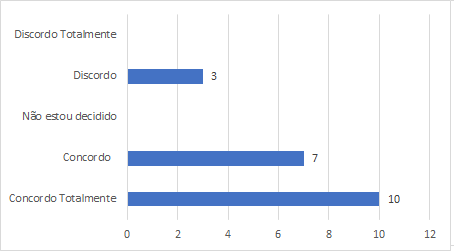
\includegraphics[scale=0.7]{figuras das questoes/3.1.png}
\caption{Preocupo-me com uso de criptografia para a proteção das informações sensíveis durante a comunicação em dispositivos móveis.}
\end{figure}

\begin{figure}[!t]
\centering
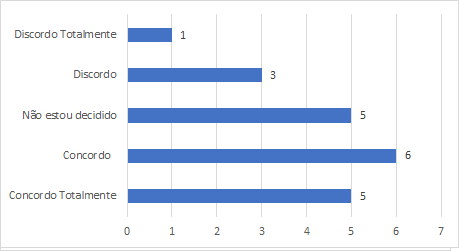
\includegraphics[scale=0.7]{figuras das questoes/3.2.png}
\caption{Preocupo-me em gerar chaves para diferentes sistemas criptográficos e diferentes aplicações.}
\end{figure}

\begin{figure}[!t]
\centering
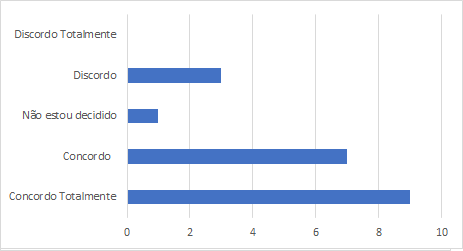
\includegraphics[scale=0.7]{figuras das questoes/4.1.png}
\caption{Preocupo-me com os impactos na segurança da informação quando ocorre alguma mudança no sistema.}
\end{figure}

\begin{figure}[!t]
\centering
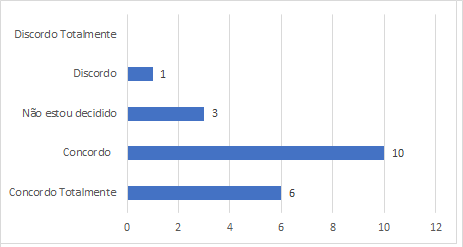
\includegraphics[scale=0.7]{figuras das questoes/4.2.png}
\caption{Preocupo-me em criar mecanismos para atender o crescimento da aplicação e possibilitar suportar demanda variável de acessos.}
\end{figure}

\begin{figure}[!t]
\centering
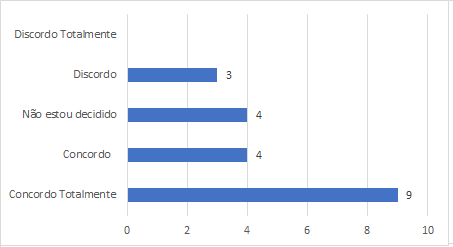
\includegraphics[scale=0.7]{figuras das questoes/4.3.png}
\caption{Preocupo-me para que dados sensíveis não sejam copiados para os ambientes de testes.}
\end{figure}

\begin{figure}[!t]
\centering
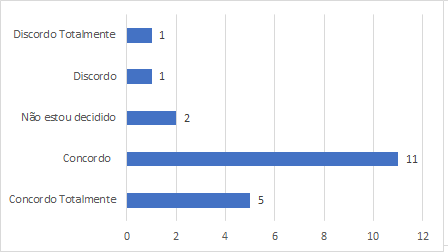
\includegraphics[scale=0.7]{figuras das questoes/5.1.png}
\caption{Preocupo-me em criar mecanismos para registrar os eventos do sistema.}
\end{figure}

\begin{figure}[!t]
\centering
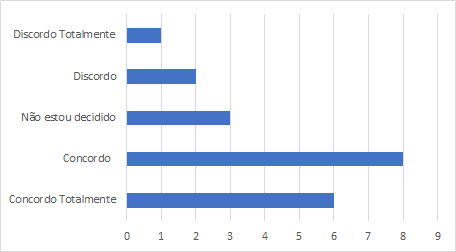
\includegraphics[scale=0.7]{figuras das questoes/5.2.png}
\caption{Preocupo-me com datas, horários e detalhes de eventos-chave, como, por exemplo, horário de entrada (log-on) e saída (log-off) no sistema.}
\end{figure}

\begin{figure}[!t]
\centering
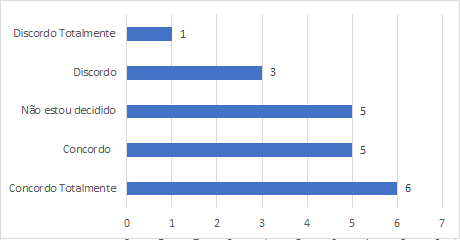
\includegraphics[scale=0.7]{figuras das questoes/5.3.png}
\caption{Preocupo-me com a identificação do dispositivo ou sua localização quando possível e o identificador do sistema.}
\end{figure}

\begin{figure}[!t]
\centering
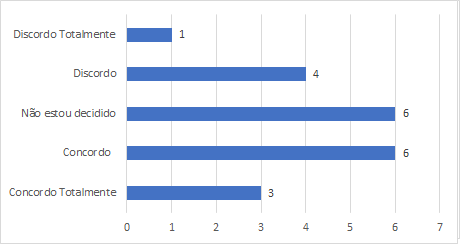
\includegraphics[scale=0.7]{figuras das questoes/5.4.png}
\caption{Preocupo-me com registro de tentativas de acesso ao sistema, aceitas e rejeitadas.}
\end{figure}
 
\begin{figure}[!t]
\centering
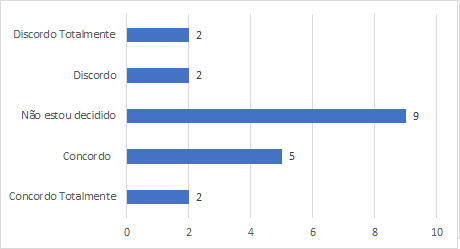
\includegraphics[scale=0.7]{figuras das questoes/5.5.png}
\caption{Preocupo-me com a coleta dos endereços e protocolos de rede no log.}
\end{figure}
 
\begin{figure}[!t]
\centering
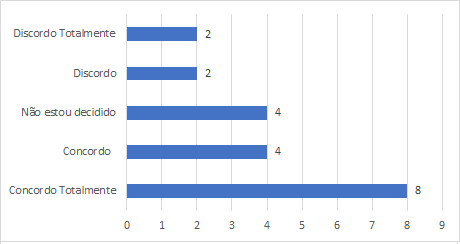
\includegraphics[scale=0.7]{figuras das questoes/5.6.png}
\caption{Preocupo-me para que arquivos de log não sejam editados ou excluídos sem a devida autorização.}
\end{figure}
   
\begin{figure}[!t]
\centering
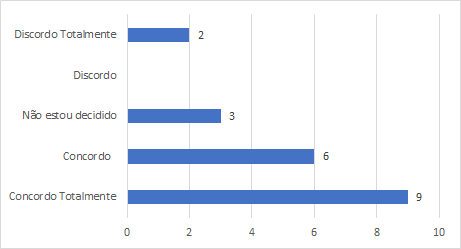
\includegraphics[scale=0.7]{figuras das questoes/6.1.png}
\caption{Preocupo-me em identificar falhas de segurança nas aplicações móveis que dou manutenção.}
\end{figure}

\begin{figure}[!t]
\centering
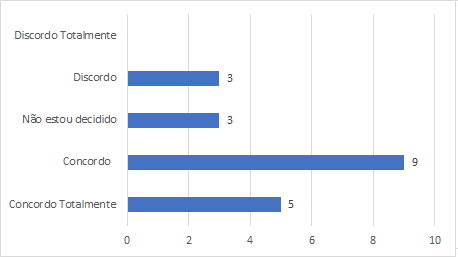
\includegraphics[scale=0.7]{figuras das questoes/6.2.png}
\caption{Respostas questão 6.2}
\end{figure}

\begin{figure}[!t]
\centering
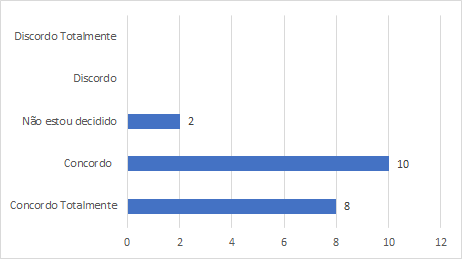
\includegraphics[scale=0.7]{figuras das questoes/6.3.png}
\caption{Respostas questão 6.3}
\end{figure}

\begin{figure}[!t]
\centering
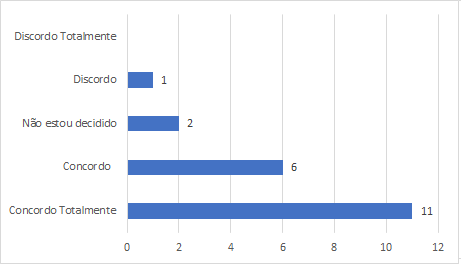
\includegraphics[scale=0.7]{figuras das questoes/6.4.png}
\caption{Respostas questão 6.4}
\end{figure}

\begin{figure}[!t]
\centering
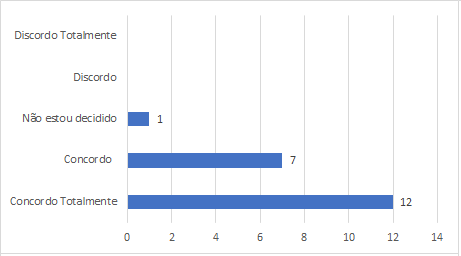
\includegraphics[scale=0.7]{figuras das questoes/6.5.png}
\caption{Respostas questão 6.5}
\end{figure}

\begin{figure}[!t]
\centering
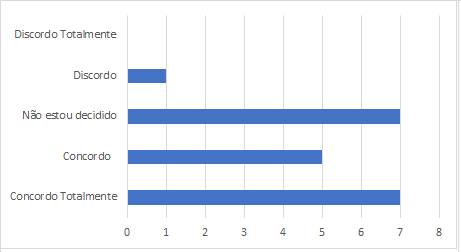
\includegraphics[scale=0.7]{figuras das questoes/6.6.png}
\caption{Respostas questão 6.6}
\end{figure}

\begin{figure}[!t]
\centering
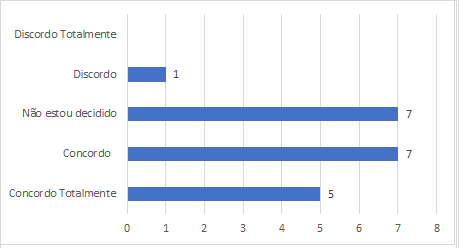
\includegraphics[scale=0.7]{figuras das questoes/6.7.png}
\caption{Respostas questão 6.7}
\end{figure}

\begin{figure}[!t]
\centering
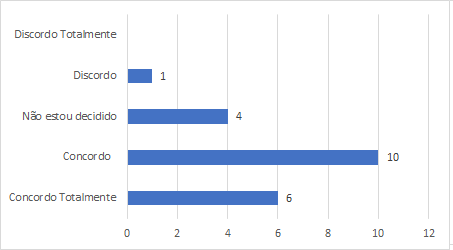
\includegraphics[scale=0.7]{figuras das questoes/6.8.png}
\caption{Respostas questão 6.8}
\end{figure}

\begin{figure}[!t]
\centering
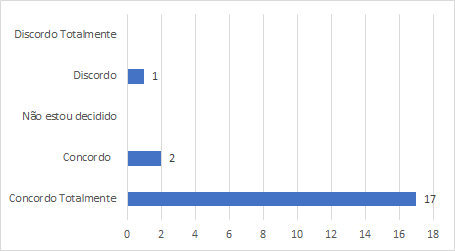
\includegraphics[scale=0.7]{figuras das questoes/6.9.png}
\caption{Respostas questão 6.9}
\end{figure}

\begin{figure}[!t]
\centering
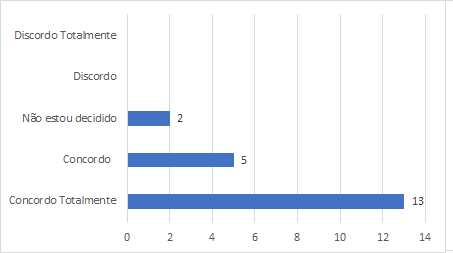
\includegraphics[scale=0.7]{figuras das questoes/6.10.png}
\caption{Respostas questão 6.11}
\end{figure}

\begin{figure}[!t]
\centering
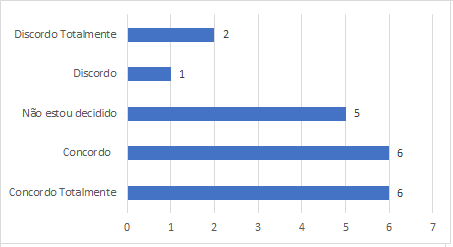
\includegraphics[scale=0.7]{figuras das questoes/6.11.png}
\caption{Respostas questão 6.11}
\end{figure}

\begin{figure}[!t]
\centering
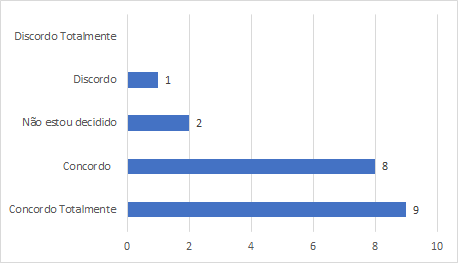
\includegraphics[scale=0.7]{figuras das questoes/6.12.png}
\caption{Respostas questão 6.12}
\end{figure}

\begin{figure}[!t]
\centering
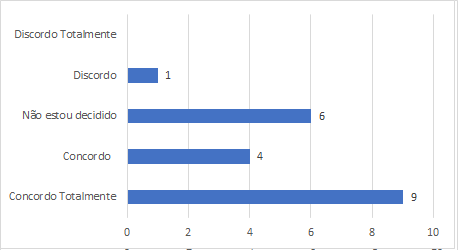
\includegraphics[scale=0.7]{figuras das questoes/6.13.png}
\caption{Respostas questão 6.13}
\end{figure}

\begin{figure}[!t]
\centering
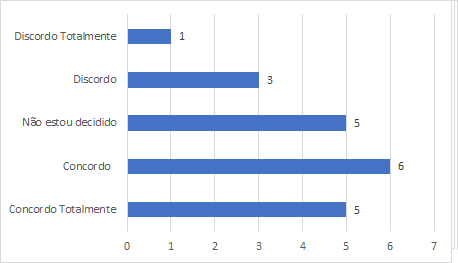
\includegraphics[scale=0.7]{figuras das questoes/6.14.png}
\caption{Respostas questão 6.14}
\end{figure}

\begin{figure}[!t]
\centering
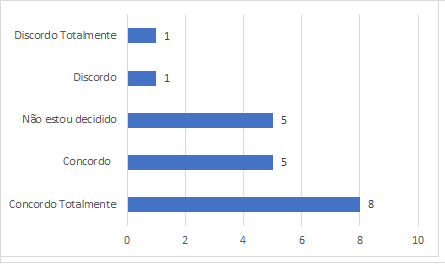
\includegraphics[scale=0.7]{figuras das questoes/6.15.png}
\caption{Respostas questão 6.15}
\end{figure}

\begin{figure}[!t]
\centering
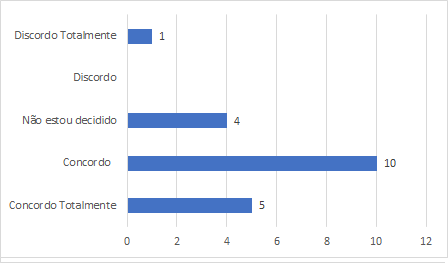
\includegraphics[scale=0.7]{figuras das questoes/6.16.png}
\caption{Respostas questão 6.16}
\end{figure}

\begin{figure}[!t]
\centering
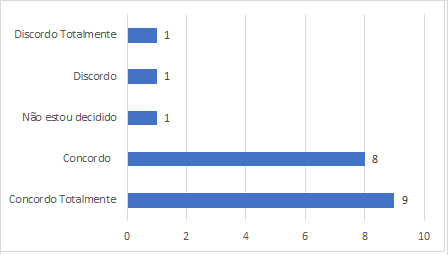
\includegraphics[scale=0.7]{figuras das questoes/6.17.png}
\caption{Respostas questão 6.17}
\end{figure}
\begin{itemize}
%\item Especialista 2: Confirmou-se com o especialista que será realizada a entrevista para examinar a qualidade das perguntas elaboradas com o especialista 1.
\end{itemize}


 

 

 
